\section{Parser generator}\label{sec:parsergenerator}
Instead of writing code by hand, several tools automatically generate code for scanning and parsing based on a grammar. \feedback{the way you put it sounds like: “we don’t feel like writing code, then we use a parser generator”. Maybe there are some deeper reasons why it’s best to employ a parser generator in contrast to implementing your own ad hoc parser} Therefore, a discussion of \textit{JavaCC}, \textit{ANTLR4}, and \textit{CUP} precedes the formal language description. The tools mentioned are only a few of those available and have been chosen because the group has experience with them through coursework.  The main reason a parser generator has been chosen is because of the gains in productivity that it makes possible. It also makes it possible to create a functioning compiler yet still have language design as a larger focus.  \supervisor{Perhaps mention that the biggest advantage of auto-generating a scanner and parser is productivity?}


Each tool is evaluated using a reduced fragment of the Bims grammar from table \ref{tab:bimsgrammar} \cite{Huttel2010}. For each tool, the grammar was adapted, and the tool was run with the rewritten grammar as input. The process of rewriting, inputting, and running the tool was compared, and a tool was selected.


\begin{table}[htb!]
    \centering
    \begin{tabular}{l}
    $n \in \textbf{Num} - \text{Numerals}$\\
    $x \in \textbf{Var} - \text{Variables}$\\
    $a \in \textbf{Aexp} - \text{Arithmetic expressions}$\\
    $b \in \textbf{Bexp} - \text{Boolean expressions}$\\
    $S \in \textbf{Stm} - \text{Statements}$\\
    \end{tabular}
    \begin{align*}
    S & \rightarrow  x \coloneqq a \mid \text{skip} \mid S_1;S_2\\
    b & \rightarrow a_1 = a_2 \mid a_1 < a_2 \mid \neg b_1 \mid b_1 \land b_2 \mid (b_1)\\
    a & \rightarrow n \mid a_1 + a_2 \mid a_1 * a_2 \mid a_1 - a_2 \mid (a_1)
    \end{align*}
    \caption{Sample Bims syntax \cite{Huttel2010}}
    \label{tab:bimsgrammar}
\end{table}


\subsection{JavaCC}
JavaCC stands for Java Compiler Compiler and is an open-source parser generator and lexical analyzer developed by Oracle, written in the Java language. It is one of the most popular parser generators for Java\cite{JavaCC2021}, and it is very well documented.

JavaCC takes as input a Context-Free Grammar (CFG) in Extended Backus-Naur Form (EBNF) to generate a scanner and a parser based on the input. The parser generated is a Left-to-right, Leftmost derivation with 1 token lookahead (LL(1)) parser by default. However, the parser can be extended to \textit{k} lookahead for parts of the grammar if necessary \cite{JavaCC2021}.

Setting up JavaCC was easy as it is well documented, and requires Java to be installed. Having set this up, we were able to begin writing our grammar. After setting up, it became clear that writing grammars in JavaCC were simple but less intuitive. In JavaCC, the grammar has to be written as code, whereas the syntax of other tools resembles the way it is seen in books, as shown in Table \ref{tab:bimsgrammar}. An example of this can be seen in listing \ref{List:javaCC}

\begin{listing}[htb!]
\centering
\begin{minted}{c}
PARSER_BEGIN(Example)

public class Example {
  public static void main(String args[]) throws ParseException {
    Example parser = new Example(System.in);
    parser.Input();
  }
}

PARSER_END(Example)

void Input() : {}
{
  MatchedBraces() ("\n"|"\r")* <EOF>
}

void MatchedBraces() : {}
{
  "{" [ MatchedBraces() ] "}"
}
\end{minted}
\caption{An example of the JavaCC syntax}
\label{List:javaCC}
\end{listing}

\subsubsection{Rewriting Bims}
Because the generated parser is LL(1), the input grammar must be non-left-recursive. Bims, however, is left-recursive and has to be rewritten. This can be seen in Table \ref{tab:bimsrewrite}.

\todo[inline]{Grammar in table is incomplete}


\begin{table}[htb!]
\centering
    \begin{align*}
    S  & \rightarrow  x \coloneqq a S' \mid \text{skip } S' \mid \text{while } S'\\
    S' & \rightarrow \text{;} S S'\mid \epsilon\\
    b  & \rightarrow a_1 = a_2 \mid a_1 < a_2 \mid \neg b_1 \mid b_1 \land b_2 \mid (b_1)\\
    a  & \rightarrow n \mid a_1 + a_2 \mid a_1 * a_2 \mid a_1 - a_2 \mid (a_1)
    \end{align*}
    \caption{Rewrite of Bims without left recursion}
    \label{tab:bimsrewrite}
\end{table}

\feedback{this part has left recursion (see comment for details).}

\subsection{ANTLR4}

ANTLR (short for ANother Tool for Language Recognition) is a powerful parser generator that can be used to process, execute, or even translate structured text or binary files. It is widely used around the world by both Twitter and Oracle for parsing queries. \cite{ANTLR_About}

One of the major advantages of ANTLR is their high level of support in almost any popular IDE, making it easy to work with regardless of the preferred development environment of the programmer. The ability to generate the lexer, parser and concrete syntax tree from a single grammar file is also very appealing. The grammar is very similar to that of EBNF and utilises a custom parsing technology called Adaptive LL(*) or ALL(*). This differs from the LL(*) used in ANTLR3, by analysing the grammar dynamically at runtime rather than statically, before the parser executes \cite{Parr2014}.

ANTLR is very easy to work with. One simply installs the plugin in their IDE of choice and read through the simple-to-understand documentation found on the official GitHub page of ANTLR \cite{ANTLR_Documentation}. Understanding the grammar rules and how to set it up in its respective grammar4 (.g4 file extension) is very manageable thanks to this. After the grammar file has been written it is possible to run the ANTLR tool on it, which then automatically generate a number of files for us, such as a parser, a lexer and a set of tokens. Then the generated code can be compiled against the ANTLR runtime. This also provides the developer with both a visual representation of the created parse tree or a tree in a LISP-like text form, along with a list of tokens found - all of these options are accessible through optional flags during compilation. The fourth major version of ANTLR introduces a lot of new capabilities compared to that of ANTLR3, which helps to reduce the learning curve by making the development of grammars and language applications easier - in part thanks to the powerful extensions and tools included in their plugins.



\subsection{CUP}
"CUP stands for Construction of Useful Parsers and is a Look-Ahead Left-to-right, Rightmost derivation (LALR) parser generator for Java" \cite{cupParserGenerator}. CUP implements a standard LALR(1) parser generation. Documentation for CUP recommends using the scanner generator JFlex, as a Lexical Analyzer Generator. Figure \ref{fig:cup_example} is an example of how CUP was used.


\begin{figure}[htb!]
    \centering
    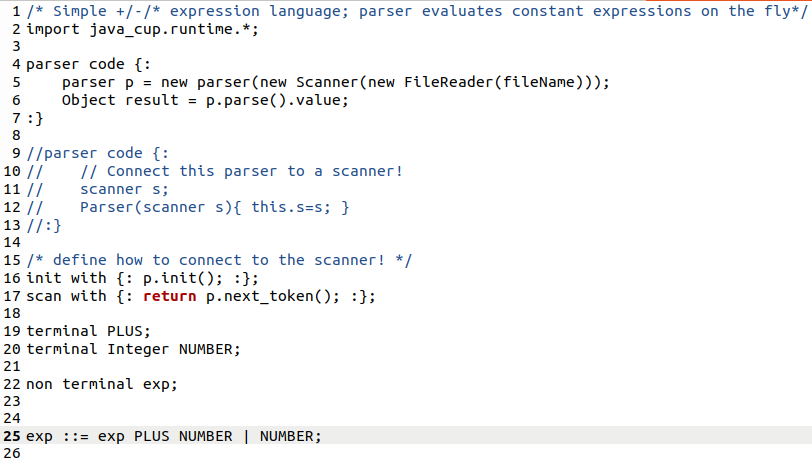
\includegraphics[scale = 0.5]{figures/Cup_Example.png}
    \caption{An example of CUP}
    \label{fig:cup_example}
\end{figure}

In this we created a simple grammar that could add two integers together; this was done to try using CUP and to understand how everything worked.


\subsubsection{JFlex}
JFlex is an abbreviation for Java Flex. Flex is an abbreviation for Fast Lexical Analyzer Generator. As the name suggests, it is a tool for generating fast lexers. It makes adjustments to the size and speed of the generated lexer possible. 

In figure \ref{fig:JFlex_example} there is an example of how JFlex looked, in conjunction with our previously mentioned CUP file. 

\begin{figure}[htb!]
    \centering
    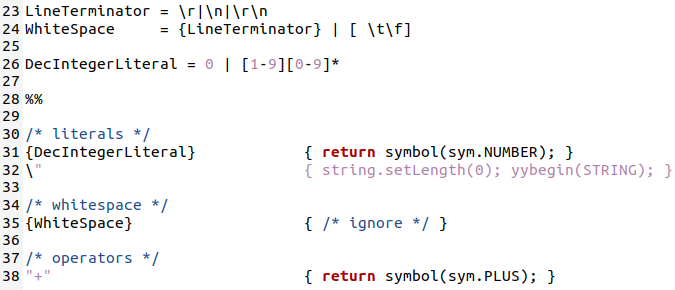
\includegraphics[scale = 0.5]{figures/JFlex_Example.png}
    \caption{An example of JFlex}
    \label{fig:JFlex_example}
\end{figure}

\subsection{Experiences with CUP}
The general experience with CUP was good, except for connecting the parser and the lexical analyzer. At first, CUP was easy and workable, and setting up a simple grammar and creating the parser and symbol tree for it went well. But when there were specific issues it was difficult to find solutions, as CUP is not a very popular parser generator, which meant there was a minimal amount of information to be found.

\subsection{Result}
\supervisor{Incomplete argumentation. Comments welcome but not necessary}
CUP will not be used in the project, as it proved difficult, combined with a lack of documentation, to connect the parser generator with the lexical analyzer generator, whereas other tools, such as JavaCC and ANTLR, automatically creates the lexical analyzer. 


Based on our experiences with the different compiler compilers we have chosen to work with ANTLR. We chose ANTLR primarily because of how powerful it is and the great extensions it provides. These factors in particular could help us to efficiently develop our language and compiler. It does commit us to a LL parser which is not as expressive as an LR parser but we do not believe this will be a problem for our language since it will be relatively compact.

%The experiences with JavaCC and ANTLR were similar. Installation was 

%JavaCC and ANTLR are very similar. Therefore the deciding factors was ANTLR's powerful tooling and simpler syntax. This meant ANTLR was chosen even though Javacc had better documentation.  